
\begin{frame}{Producing Climate Projections}
  \begin{tikzpicture}[
      remember picture,
      overlay,
      process/.style={-{Latex[length=2.6mm,width=2.2mm]},
      draw=black,fill=accent2,line width=0.7pt}
    ]
    \node[anchor=north west,inner sep=0pt] (gcm) at
    ([xshift=1.35cm,yshift=-1.65cm]current page.north west)
    {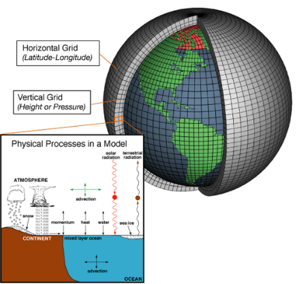
\includegraphics[width=3.35cm]{images/climate_models/global_climate_model.png}};
    \node[anchor=south east,font=\fontsize{3.1}{3.4}\selectfont] at
    ([xshift=-0.05cm,yshift=0.08cm]gcm.south east)
    {Source: NOAA.com};

    \node[anchor=north east,inner sep=0pt] (scenarios) at
    ([xshift=-0.75cm,yshift=-1.80cm]current page.north east)
    {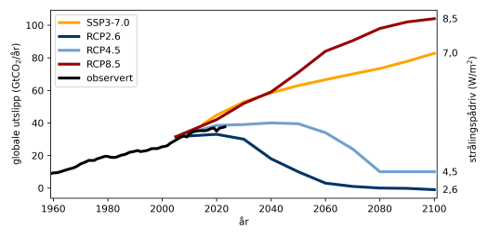
\includegraphics[width=5.15cm]{images/climate_models/klima_i_norge_scenarioer.png}};
    \node[anchor=south,font=\bfseries\scriptsize] at
    ([yshift=0.0cm]scenarios.north) {Global CO$_2$ emission scenarios};
    \node[anchor=north east,font=\fontsize{4.2}{4.6}\selectfont] at
    ([yshift=-0.0cm]scenarios.south east)
    {From the report \textit{Klima i Norge} (2025)};

    \node[anchor=south,inner sep=0pt] (downscaling) at
    ([xshift=-0.10cm,yshift=0.18cm]current page.south)
    {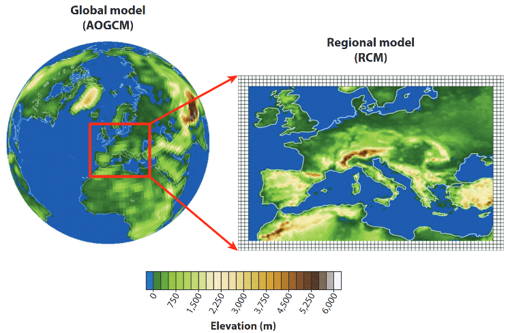
\includegraphics[width=6.05cm]{images/climate_models/regional_climate_model.png}};
    \node[anchor=south east,align=left,text width=1.72cm,
    font=\fontsize{3.1}{3.4}\selectfont] at
    ([xshift=-0.04cm,yshift=0.07cm]downscaling.south east)
    {From: F. Giorgi and W. Gutowski (2015):\\
    \textit{Regional Dynamical Downscaling and the CORDEX Initiative}};

    \node[anchor=south east,inner sep=0pt] (bias) at
    ([xshift=-0.40cm,yshift=0.80cm]current page.south east)
    {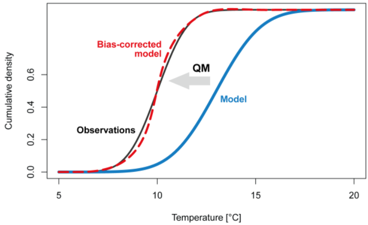
\includegraphics[width=3.95cm]{images/climate_models/bias_correction.png}};
    \node[anchor=south,font=\bfseries\scriptsize] at
    ([yshift=0.10cm]bias.north) {Bias correction};
    \node[anchor=north east,align=left,
    font=\fontsize{3.1}{3.4}\selectfont] at
    ([xshift=-0.02cm,yshift=+0.1cm]bias.south east)
    {From: MeteoSwiss\\tech rep no 270};

    \draw[process] ([xshift=0.30cm,yshift=-0.28cm]gcm.east) --
    ([xshift=-0.55cm,yshift=0.22cm]downscaling.north);
    \draw[process] (scenarios.west) --
    ([xshift=-2.45cm,yshift=+0.1cm]downscaling.north east);
    \draw[process] ([xshift=0.15cm,yshift=0.5cm]downscaling.east) --
    ([xshift=-0.20cm,yshift=0.25cm]bias.west);

    \node[anchor=south west,align=left,font=\small] (uncertainty) at
    ([xshift=1.25cm,yshift=1.1cm]current page.south west)
    {Complex model\\decisions,\\uncertainty in\\calibration data};
  \end{tikzpicture}
\end{frame}

\begin{frame}{Change the climate, hold building portfolio fixed}
  \vspace{0.5cm}
  \centering
  \begin{tikzpicture}[
      period/.style={draw=accent1,thick,rounded corners=2pt,fill=softgrey,
      minimum width=3.4cm,minimum height=1.45cm,text width=3.0cm,align=center},
      future/.style={draw=riskred,thick,rounded corners=2pt,fill=white,
      minimum width=3.4cm,minimum height=1.45cm,text width=3.0cm,align=center},
      arrow/.style={-{Latex[length=3mm]},thick,color=accent1}
    ]
    \node[period] (base) at (-4.3,0) {\textbf{Reference}\\1991--2020};
    \node[future] (mid) at (0,0) {\textbf{Mid-century}\\2041--2070};
    \node[future] (late) at (4.3,0) {\textbf{Late century}\\2071--2100};
    \draw[arrow] (base) -- (mid);
    \draw[arrow] (mid) -- (late);
    \node[below=0.5cm of base,align=center] {Same portfolio\\and 2026 prices};
    \node[below=0.5cm of mid,align=center] {RCP2.6\\RCP4.5\\SSP3-7.0};
    \node[below=0.5cm of late,align=center] {RCP2.6\\RCP4.5\\SSP3-7.0};
  \end{tikzpicture}

  \vspace{0.45cm}
  \textbf{10 climate simulations $\times$ 2 bias adjustments $\times$
  10 posterior draws}

  \vspace{0.15cm}
  = 200 relative cost changes per scenario, horizon, and geography
  \sourceNote{Norwegian Climate Service Centre projections released in 2025}
\end{frame}

\begin{frame}{National change in total damages}
  \captionsetup{labelformat=empty,font=footnotesize}
  \vspace{0.4cm}
  \begin{table}
    \centering
    \footnotesize
    \setlength{\tabcolsep}{6pt}
    \renewcommand{\arraystretch}{1.35}
    \makebox[\linewidth][c]{
      \begin{tabular}{llccc}
        \shortstack{\textbf{Future} \\ \textbf{period}} &
        \shortstack{\textbf{Emissions} \\ \textbf{scenario}} &
        \shortstack{\textbf{Lower} \\ \textbf{quartile}} &
        \textcolor{accent1}{\textbf{Median}} &
        \shortstack{\textbf{Upper} \\ \textbf{quartile}} \\
        \hline
        2041--2070 & Low & \(7.1\%\) &
        \textcolor{accent1}{\(\mathbf{9.5\%}\)} & \(17.5\%\) \\
        & Intermediate & \(10.2\%\) &
        \textcolor{accent1}{\(\mathbf{14.9\%}\)} & \(22.9\%\) \\
        & High & \(11.1\%\) &
        \textcolor{accent1}{\(\mathbf{18.3\%}\)} & \(22.8\%\) \\
        \hline
        2071--2100 & Low & \(6.4\%\) &
        \textcolor{accent1}{\(\mathbf{9.9\%}\)} & \(18.0\%\) \\
        & Intermediate & \(14.7\%\) &
        \textcolor{accent1}{\(\mathbf{23.4\%}\)} & \(30.6\%\) \\
        & High & \(17.0\%\) &
        \textcolor{accent1}{\(\mathbf{33.2\%}\)} & \(41.6\%\) \\
        \hline
    \end{tabular}}
    \caption{Percent changes in total damages, across all of Norway.}
    \label{tab:national_changes}
  \end{table}
\end{frame}

% \begin{frame}{National costs rise in every scenario}
%   \begin{columns}[T,onlytextwidth]
%     \begin{column}{0.40\textwidth}
%       \begin{itemize}
%         \item Median changes are positive for every scenario, and horizon
%         \item Increases are larger under higher emissions
%         \item Scenario differences are most pronounced late in the century
%         \item Under high emissions, the late-century median is about
%           one third above the reference climate
%       \end{itemize}
%     \end{column}
%     \begin{column}{0.57\textwidth}
%       \centering
%       \scriptsize
%       \renewcommand{\arraystretch}{1.35}
%       \begin{tabular}{lrr}
%         \textbf{Scenario} & \textbf{2041--2070} & \textbf{2071--2100} \\
%         \hline
%         Low -- RCP2.6 & $+9.5\%$ & $+9.9\%$ \\
%         Intermediate -- RCP4.5 & $+14.9\%$ & $+23.4\%$ \\
%         High -- SSP3-7.0 & $+18.3\%$ & $\mathbf{+33.2\%}$
%       \end{tabular}
%       \vspace{0.45cm}
%       Medians of 200 relative cost changes
%     \end{column}
%   \end{columns}
%   \sourceNote{Reference period 1991--2020}
% \end{frame}
% \begin{frame}{Emissions matter most late in the century}
%   \begin{columns}[T,onlytextwidth]
%     \begin{column}{0.48\textwidth}
%       \begin{itemize}
%         \item Scenario medians are closer at mid-century
%         \item They diverge substantially by 2071--2100
%         \item Climate-model differences dominate much of the ensemble spread
%         \item Ensemble quantiles are not calibrated probabilities
%       \end{itemize}
%     \end{column}
%     \begin{column}{0.47\textwidth}
%       \textbf{High emissions, 2071--2100}
%       \vspace{0.25cm}
%       \begin{tabular}{lr}
%         10th percentile & $+10.1\%$ \\
%         Lower quartile & $+17.0\%$ \\
%         Median & $+33.2\%$ \\
%         Upper quartile & $+41.6\%$ \\
%         90th percentile & $+46.8\%$
%       \end{tabular}
%     \end{column}
%   \end{columns}
%   \sourceNote{National projection ensemble}
% \end{frame}

\begin{frame}{Impact geographically uneven}
  \begin{columns}[T,onlytextwidth]
    \begin{column}{0.48\textwidth}
      \vspace{1cm}
      \begin{itemize}
        \item High-emissions county medians:
          \begin{itemize}\footnotesize
            \item 2041--2070: ca.\ $+8$ to $+25\%$
            \item 2071--2100: ca.\ $+17$ to $+61\%$
          \end{itemize}
        \item Largest increases in Finnmark and southern mountain regions
        \item Lower increases in Western Norway
      \end{itemize}
    \end{column}
    \begin{column}{0.49\textwidth}
      % Replace with an English-labelled county figure using the same filename.
      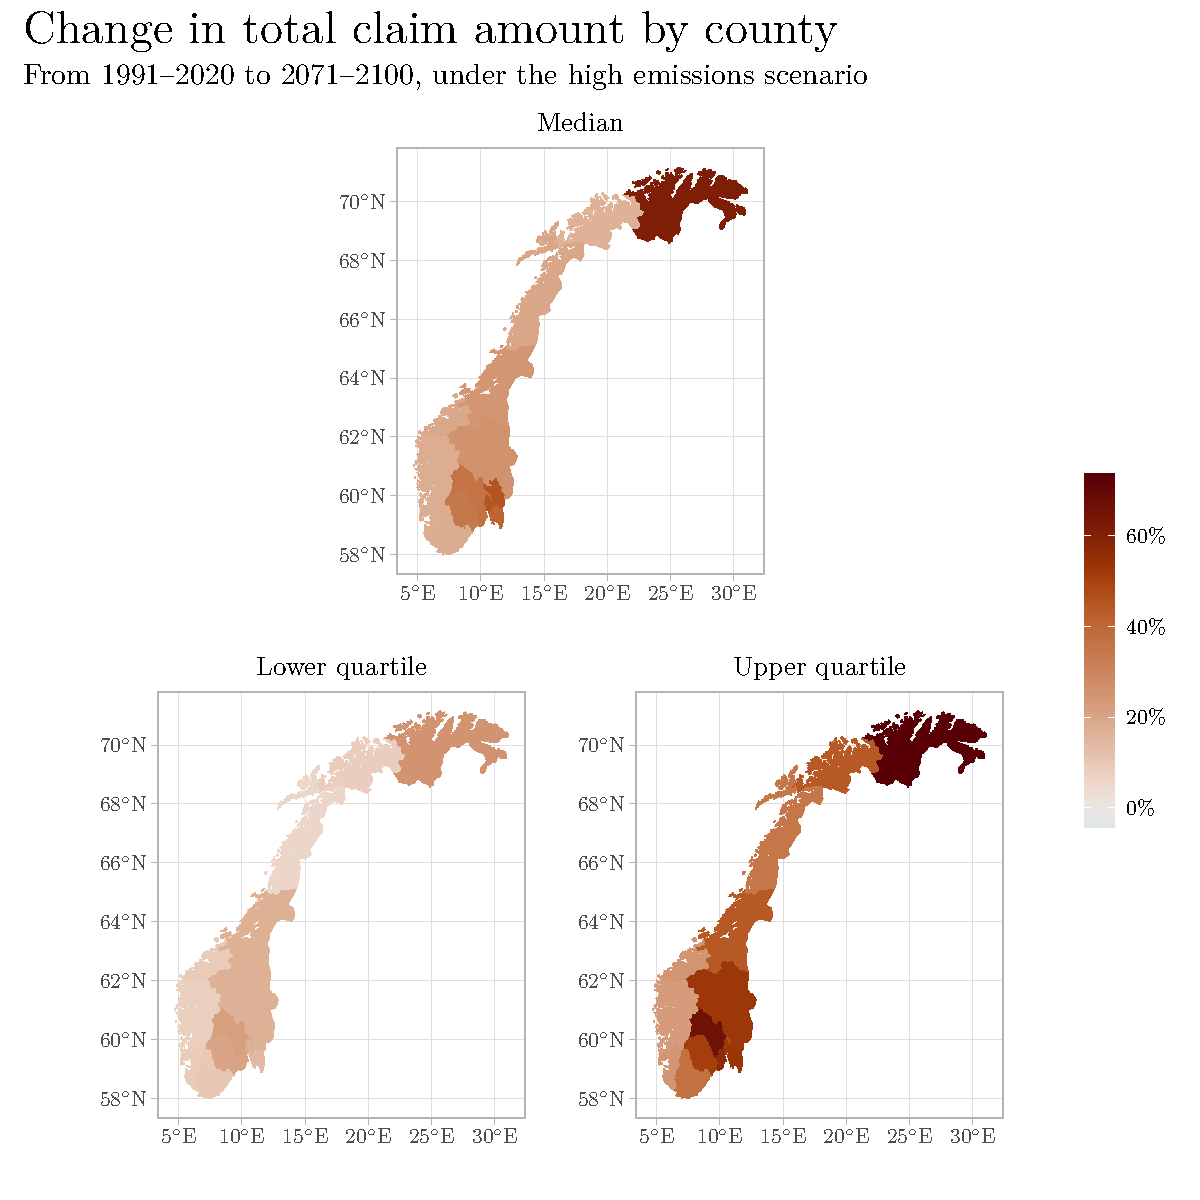
\includegraphics[width=\linewidth,height=0.72\textheight,keepaspectratio]{images/claim_simulations/quartile_county_changes_total_claim_amount_high_late_century.pdf}
    \end{column}
  \end{columns}
  \sourceNote{County medians; high-emissions scenario}
\end{frame}
% \begin{frame}{County changes under high emissions, late century}
%   \centering
%   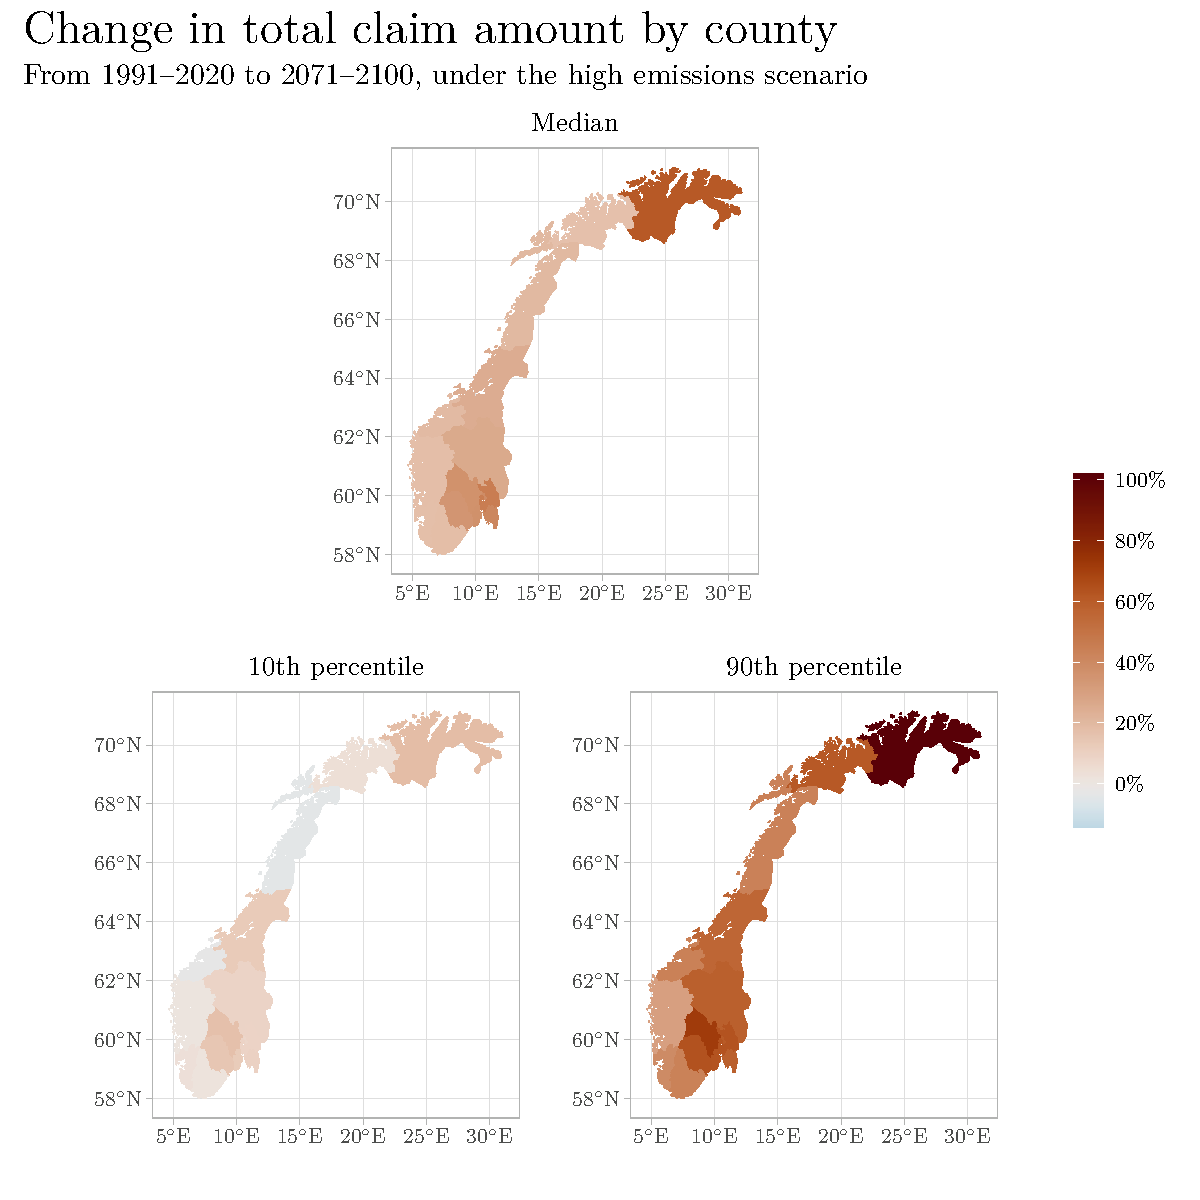
\includegraphics[width=\textwidth,height=0.78\textheight,keepaspectratio]{images/claim_simulations/quantile_county_changes_total_claim_amount_high_late_century.pdf}
% \end{frame}

\begin{frame}{Geographical spread in median impact}
  \centering
  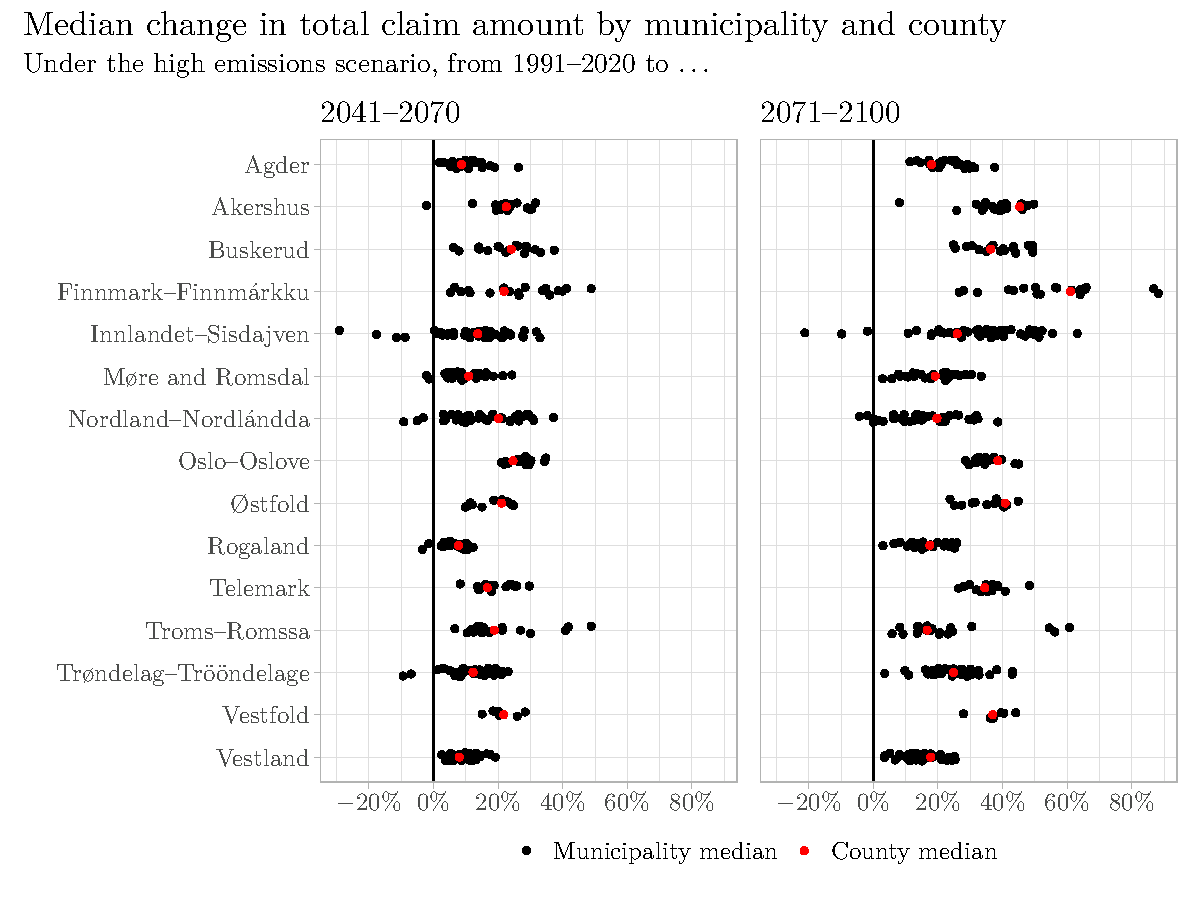
\includegraphics[width=\textwidth,height=0.78\textheight,keepaspectratio]{images/claim_simulations/county_scatter_total_claim_amount_high.pdf}
\end{frame}

\begin{frame}{Geographical spread in median impact}
  \centering
  \def\overlayCircleRadius{0.35cm}
  \def\overlayCircleOpacity{0.0}
  \begin{tikzpicture}
    \node[anchor=center,inner sep=0pt] (countyScatter) at (0,0)
    {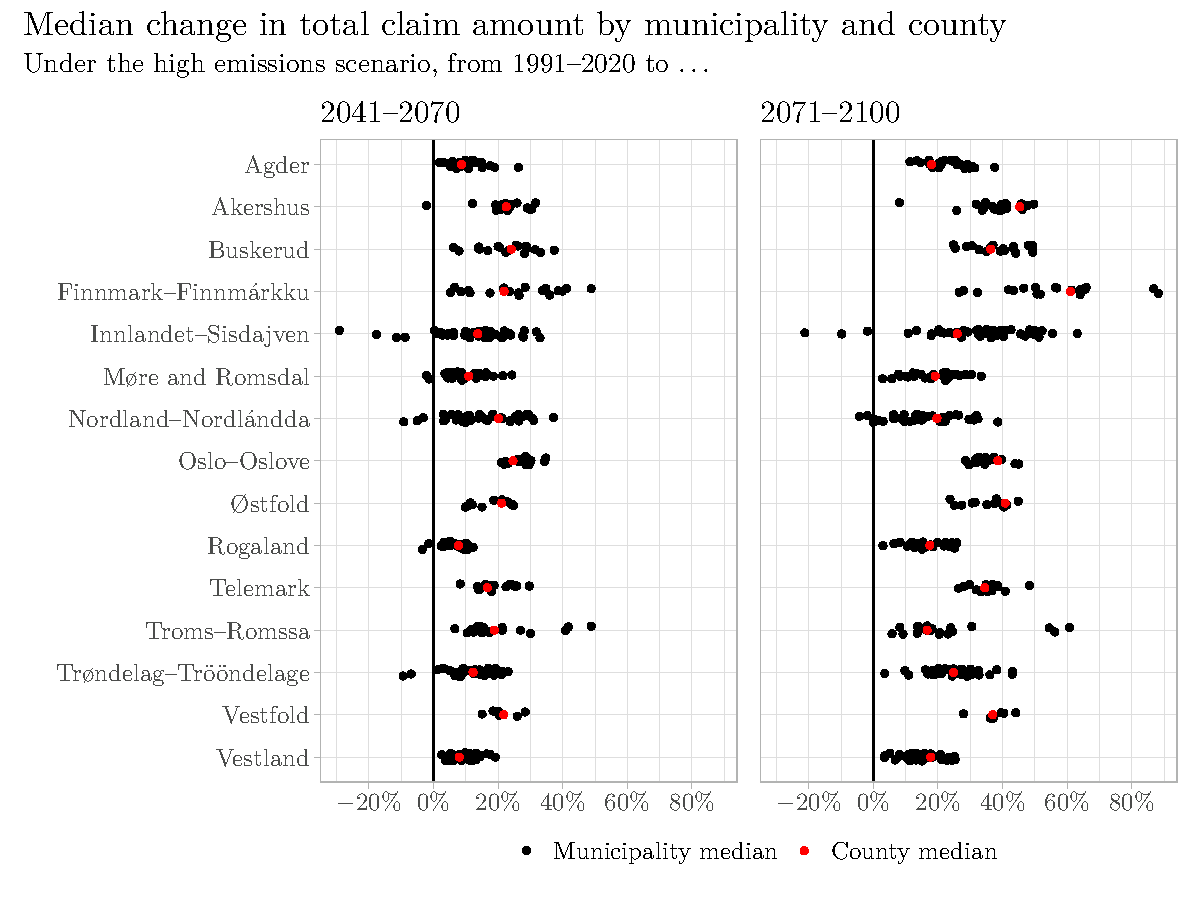
\includegraphics[width=\textwidth,height=0.78\textheight,keepaspectratio]{images/claim_simulations/county_scatter_total_claim_amount_high.pdf}};

    \coordinate (leftCircle) at
    ([yshift=-2.50cm]$(countyScatter.north
    west)!0.31!(countyScatter.north east)$);
    \coordinate (rightCircle) at
    ([yshift=-2.50cm]$(countyScatter.north
    west)!0.70!(countyScatter.north east)$);
    \filldraw[fill=white,fill opacity=\overlayCircleOpacity,
    draw=riskred,line width=1.2pt]
    (leftCircle) circle[radius=\overlayCircleRadius];
    \filldraw[fill=white,fill opacity=\overlayCircleOpacity,
    draw=riskred,line width=1.2pt]
    (rightCircle) circle[radius=\overlayCircleRadius];
  \end{tikzpicture}
\end{frame}

\begin{frame}{}
  \vspace{0.25cm}
  \centering
  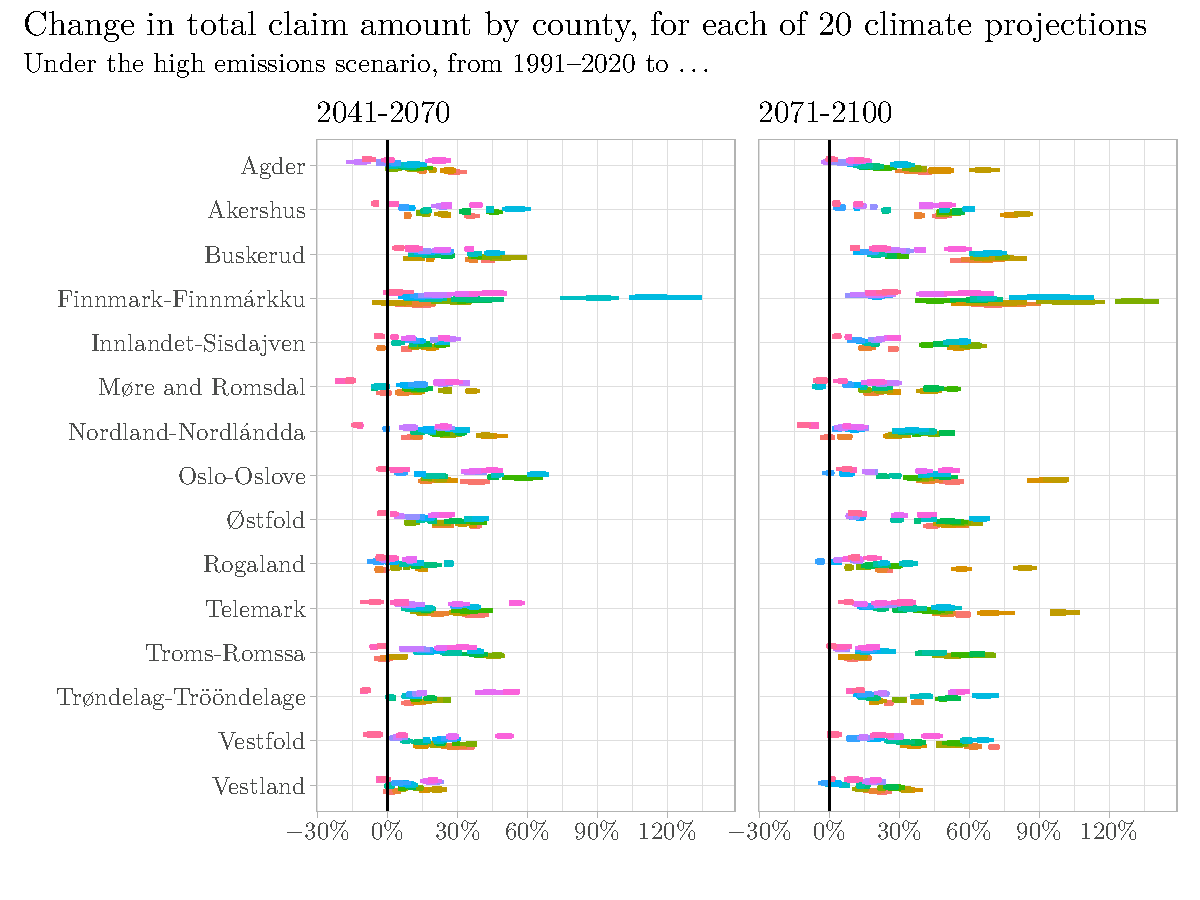
\includegraphics[width=\textwidth,height=0.93\textheight,keepaspectratio]{images/claim_simulations/county_variability_total_claim_amount_high.pdf}
\end{frame}
